\documentclass{standalone}
\usepackage{tikz}
\usetikzlibrary{patterns, positioning}
\usepackage[sfdefault]{ClearSans} %% option 'sfdefault' activates Clear Sans as the default text font
\usepackage[T1]{fontenc}

\begin{document}
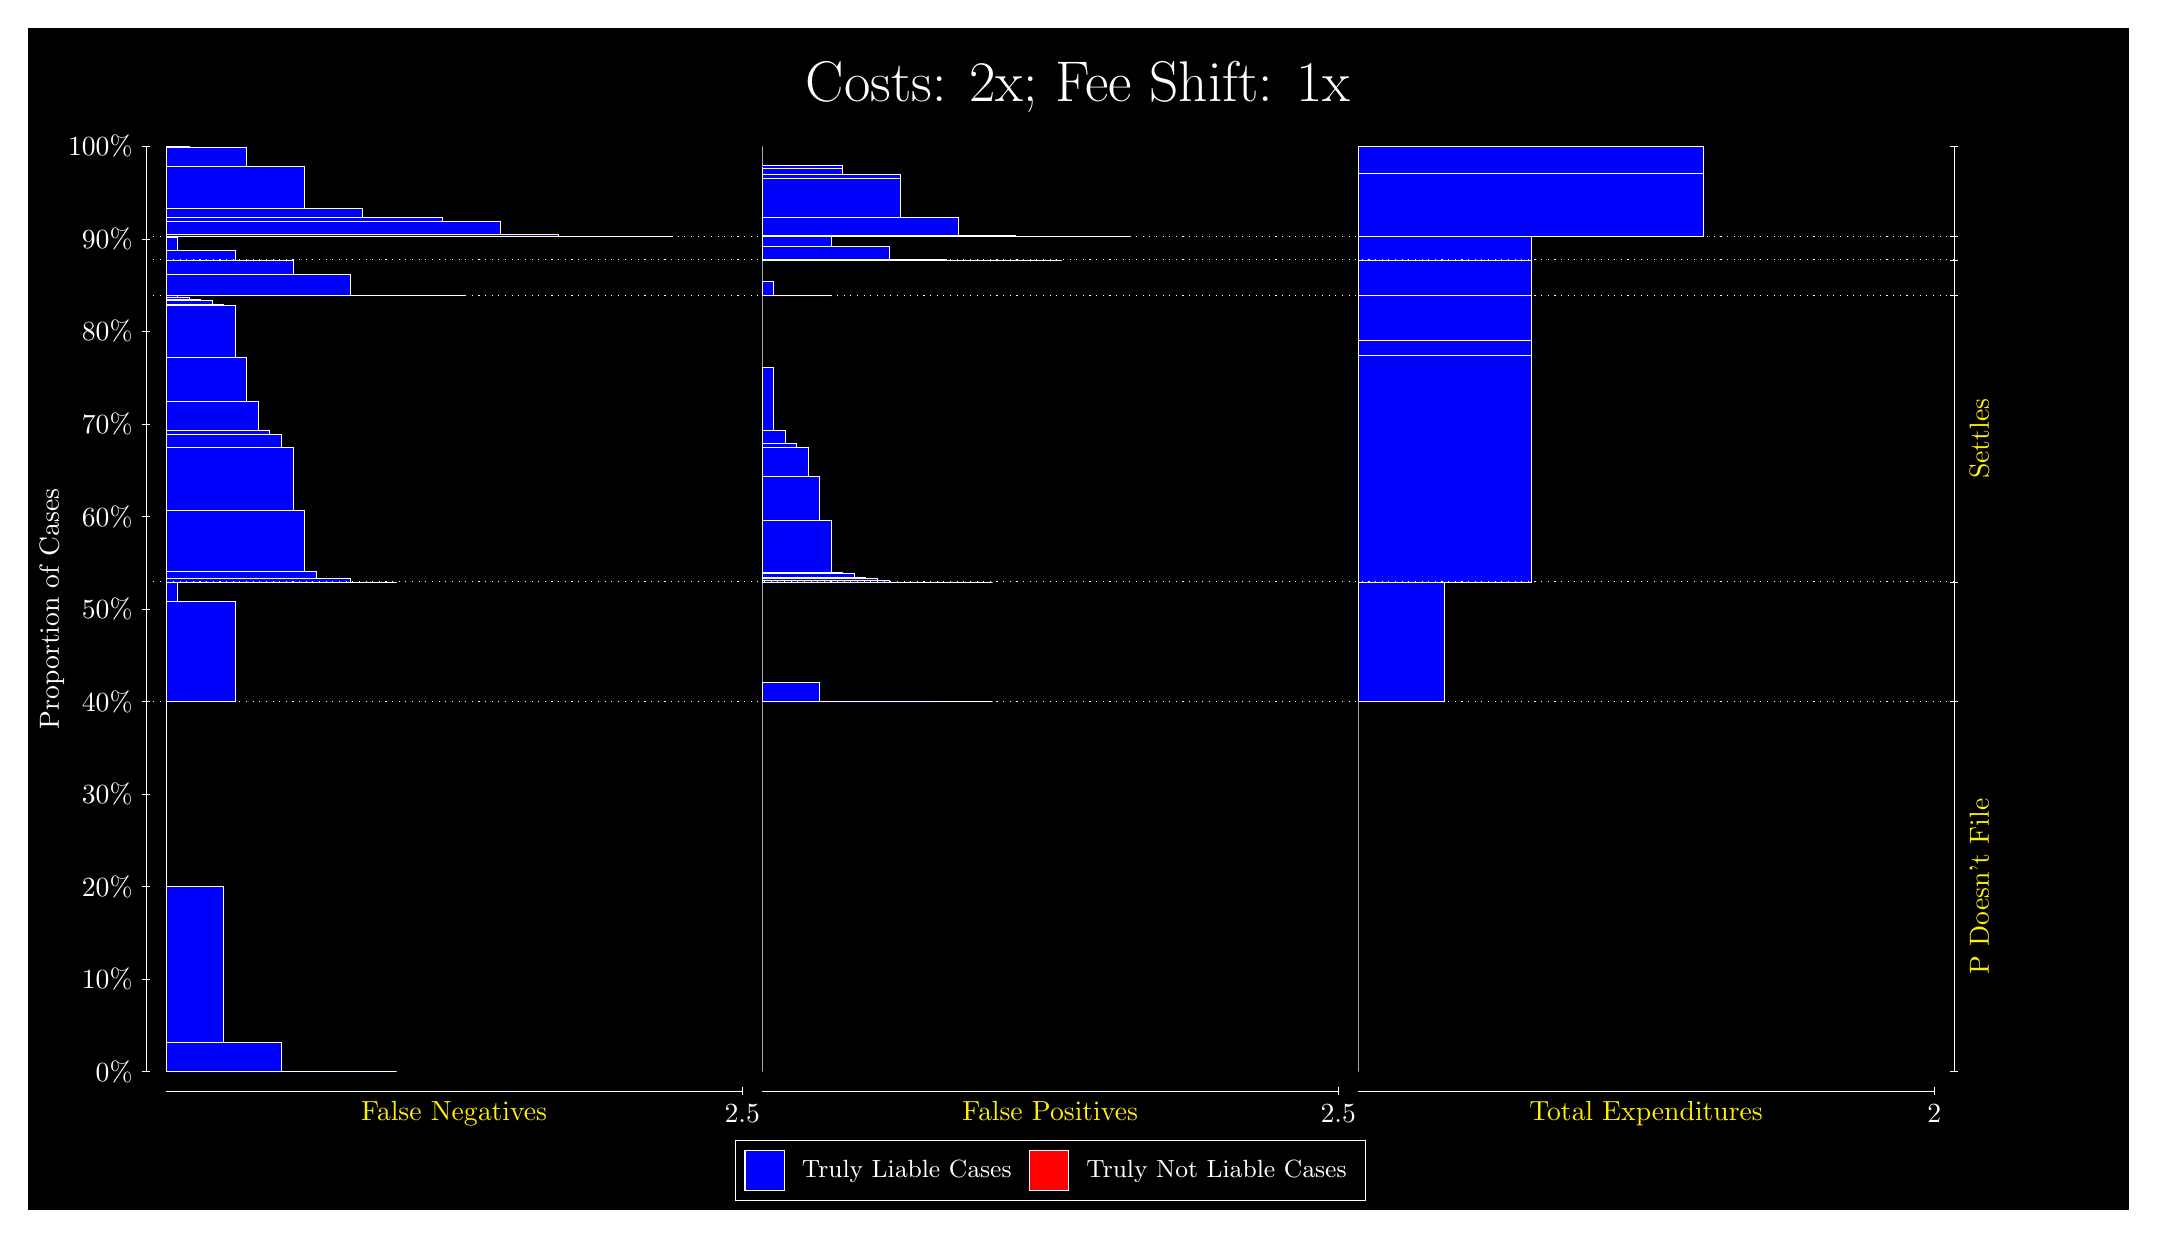
\begin{tikzpicture}
\draw[fill=black] (0,0) rectangle (26.667,15);
\draw[text=white] (0,13.5) rectangle (26.667,15) node[midway] {\huge Costs: 2x; Fee Shift: 1x};
\draw[white, very thin] (1.5,1.75) -- (1.5,13.5);
\node[rotate=90, text=white, anchor=center] at (0.3, 7.625) {Proportion of Cases};
\draw[white, very thin] (1.45,1.75) -- (1.55,1.75);
\node[text=white, anchor=east] at (1.45, 1.75) {0\%};
\draw[white, very thin] (1.45,2.925) -- (1.55,2.925);
\node[text=white, anchor=east] at (1.45, 2.925) {10\%};
\draw[white, very thin] (1.45,4.1) -- (1.55,4.1);
\node[text=white, anchor=east] at (1.45, 4.1) {20\%};
\draw[white, very thin] (1.45,5.275) -- (1.55,5.275);
\node[text=white, anchor=east] at (1.45, 5.275) {30\%};
\draw[white, very thin] (1.45,6.45) -- (1.55,6.45);
\node[text=white, anchor=east] at (1.45, 6.45) {40\%};
\draw[white, very thin] (1.45,7.625) -- (1.55,7.625);
\node[text=white, anchor=east] at (1.45, 7.625) {50\%};
\draw[white, very thin] (1.45,8.8) -- (1.55,8.8);
\node[text=white, anchor=east] at (1.45, 8.8) {60\%};
\draw[white, very thin] (1.45,9.975) -- (1.55,9.975);
\node[text=white, anchor=east] at (1.45, 9.975) {70\%};
\draw[white, very thin] (1.45,11.15) -- (1.55,11.15);
\node[text=white, anchor=east] at (1.45, 11.15) {80\%};
\draw[white, very thin] (1.45,12.325) -- (1.55,12.325);
\node[text=white, anchor=east] at (1.45, 12.325) {90\%};
\draw[white, very thin] (1.45,13.5) -- (1.55,13.5);
\node[text=white, anchor=east] at (1.45, 13.5) {100\%};

\draw[white, very thin] (24.457,1.75) -- (24.457,13.5);
\draw[white, very thin] (24.407,1.75) -- (24.507,1.75);
\node[anchor=west] at (24.407, 1.75) {};
\draw[white, very thin] (24.407,6.4489) -- (24.507,6.4489);
\node[anchor=west] at (24.407, 6.4489) {};
\draw[white, very thin] (24.407,7.9684) -- (24.507,7.9684);
\node[anchor=west] at (24.407, 7.9684) {};
\draw[white, very thin] (24.407,11.604) -- (24.507,11.604);
\node[anchor=west] at (24.407, 11.604) {};
\draw[white, very thin] (24.407,12.058) -- (24.507,12.058);
\node[anchor=west] at (24.407, 12.058) {};
\draw[white, very thin] (24.407,12.356) -- (24.507,12.356);
\node[anchor=west] at (24.407, 12.356) {};
\draw[white, very thin] (24.407,13.5) -- (24.507,13.5);
\node[anchor=west] at (24.407, 13.5) {};

\draw[white, very thin, fill=blue] (1.75,1.75) rectangle (4.6775,1.75);
\draw[white, very thin, fill=blue] (1.75,1.75) rectangle (3.9457,1.7532);
\draw[white, very thin, fill=blue] (1.75,1.7532) rectangle (3.2138,2.126);
\draw[white, very thin, fill=blue] (1.75,2.126) rectangle (2.4819,4.1027);
\draw[white, very thin, fill=red] (1.75,4.1027) rectangle (1.75,4.1027);
\draw[white, very thin, fill=blue] (1.75,4.1027) rectangle (1.75,6.4489);
\draw[white, very thin, fill=blue] (1.75,6.4489) rectangle (2.6283,7.7201);
\draw[white, very thin, fill=blue] (1.75,7.7201) rectangle (1.8964,7.9666);
\draw[white, very thin, fill=red] (1.75,7.9666) rectangle (1.75,7.9666);
\draw[white, very thin, fill=blue] (1.75,7.9666) rectangle (1.75,7.9684);
\draw[white, very thin, fill=blue] (1.75,7.9684) rectangle (4.6775,7.9684);
\draw[white, very thin, fill=blue] (1.75,7.9684) rectangle (4.3848,7.9686);
\draw[white, very thin, fill=blue] (1.75,7.9686) rectangle (4.092,8.0107);
\draw[white, very thin, fill=blue] (1.75,8.0107) rectangle (3.9457,8.0182);
\draw[white, very thin, fill=blue] (1.75,8.0182) rectangle (3.7993,8.0189);
\draw[white, very thin, fill=blue] (1.75,8.0189) rectangle (3.6529,8.1031);
\draw[white, very thin, fill=blue] (1.75,8.1031) rectangle (3.5065,8.8839);
\draw[white, very thin, fill=blue] (1.75,8.8839) rectangle (3.3602,9.684);
\draw[white, very thin, fill=blue] (1.75,9.684) rectangle (3.2138,9.8388);
\draw[white, very thin, fill=blue] (1.75,9.8388) rectangle (3.0674,9.8957);
\draw[white, very thin, fill=blue] (1.75,9.8957) rectangle (2.921,10.262);
\draw[white, very thin, fill=blue] (1.75,10.262) rectangle (2.7746,10.817);
\draw[white, very thin, fill=blue] (1.75,10.817) rectangle (2.6283,11.477);
\draw[white, very thin, fill=blue] (1.75,11.477) rectangle (2.4819,11.499);
\draw[white, very thin, fill=blue] (1.75,11.499) rectangle (2.3355,11.546);
\draw[white, very thin, fill=blue] (1.75,11.546) rectangle (2.1891,11.562);
\draw[white, very thin, fill=blue] (1.75,11.562) rectangle (2.0428,11.582);
\draw[white, very thin, fill=blue] (1.75,11.582) rectangle (1.8964,11.604);
\draw[white, very thin, fill=red] (1.75,11.604) rectangle (1.75,11.604);
\draw[white, very thin, fill=blue] (1.75,11.604) rectangle (1.75,11.604);
\draw[white, very thin, fill=blue] (1.75,11.604) rectangle (5.5558,11.604);
\draw[white, very thin, fill=blue] (1.75,11.604) rectangle (4.8239,11.611);
\draw[white, very thin, fill=blue] (1.75,11.611) rectangle (4.092,11.871);
\draw[white, very thin, fill=blue] (1.75,11.871) rectangle (3.3602,12.056);
\draw[white, very thin, fill=blue] (1.75,12.056) rectangle (2.6283,12.058);
\draw[white, very thin, fill=red] (1.75,12.058) rectangle (1.75,12.058);
\draw[white, very thin, fill=blue] (1.75,12.058) rectangle (2.6283,12.18);
\draw[white, very thin, fill=blue] (1.75,12.18) rectangle (1.8964,12.351);
\draw[white, very thin, fill=red] (1.75,12.351) rectangle (1.75,12.351);
\draw[white, very thin, fill=blue] (1.75,12.351) rectangle (1.75,12.356);
\draw[white, very thin, fill=blue] (1.75,12.356) rectangle (8.1906,12.356);
\draw[white, very thin, fill=blue] (1.75,12.356) rectangle (7.4587,12.356);
\draw[white, very thin, fill=blue] (1.75,12.356) rectangle (6.7268,12.38);
\draw[white, very thin, fill=blue] (1.75,12.38) rectangle (5.9949,12.548);
\draw[white, very thin, fill=blue] (1.75,12.548) rectangle (5.7022,12.548);
\draw[white, very thin, fill=blue] (1.75,12.548) rectangle (5.2631,12.601);
\draw[white, very thin, fill=blue] (1.75,12.601) rectangle (4.9703,12.602);
\draw[white, very thin, fill=blue] (1.75,12.602) rectangle (4.5312,12.602);
\draw[white, very thin, fill=blue] (1.75,12.602) rectangle (4.2384,12.709);
\draw[white, very thin, fill=blue] (1.75,12.709) rectangle (3.7993,12.709);
\draw[white, very thin, fill=blue] (1.75,12.709) rectangle (3.5065,13.251);
\draw[white, very thin, fill=blue] (1.75,13.251) rectangle (2.7746,13.487);
\draw[white, very thin, fill=blue] (1.75,13.487) rectangle (2.0428,13.5);
\draw[white, very thin, fill=red] (1.75,13.5) rectangle (1.75,13.5);
\draw[white, very thin, fill=blue] (1.75,13.5) rectangle (1.75,13.5);
\draw[white, very thin, fill=red] (9.3189,1.75) rectangle (9.3189,1.75);
\draw[white, very thin, fill=blue] (9.3189,1.75) rectangle (9.3189,6.4489);
\draw[white, very thin, fill=red] (9.3189,6.4489) rectangle (12.246,6.4489);
\draw[white, very thin, fill=blue] (9.3189,6.4489) rectangle (12.246,6.4489);
\draw[white, very thin, fill=blue] (9.3189,6.4489) rectangle (11.515,6.4489);
\draw[white, very thin, fill=blue] (9.3189,6.4489) rectangle (10.783,6.4507);
\draw[white, very thin, fill=blue] (9.3189,6.4507) rectangle (10.051,6.6972);
\draw[white, very thin, fill=blue] (9.3189,6.6972) rectangle (9.3189,7.9684);
\draw[white, very thin, fill=red] (9.3189,7.9684) rectangle (12.246,7.9684);
\draw[white, very thin, fill=blue] (9.3189,7.9684) rectangle (12.246,7.9684);
\draw[white, very thin, fill=red] (9.3189,7.9684) rectangle (11.954,7.9684);
\draw[white, very thin, fill=blue] (9.3189,7.9684) rectangle (11.954,7.9684);
\draw[white, very thin, fill=red] (9.3189,7.9684) rectangle (11.661,7.9684);
\draw[white, very thin, fill=blue] (9.3189,7.9684) rectangle (11.661,7.9684);
\draw[white, very thin, fill=blue] (9.3189,7.9684) rectangle (11.515,7.9684);
\draw[white, very thin, fill=red] (9.3189,7.9684) rectangle (11.368,7.9684);
\draw[white, very thin, fill=blue] (9.3189,7.9684) rectangle (11.368,7.9684);
\draw[white, very thin, fill=blue] (9.3189,7.9684) rectangle (11.222,7.9685);
\draw[white, very thin, fill=red] (9.3189,7.9685) rectangle (11.075,7.9685);
\draw[white, very thin, fill=blue] (9.3189,7.9685) rectangle (11.075,7.9685);
\draw[white, very thin, fill=blue] (9.3189,7.9685) rectangle (10.929,7.9908);
\draw[white, very thin, fill=blue] (9.3189,7.9908) rectangle (10.783,8.0106);
\draw[white, very thin, fill=blue] (9.3189,8.0106) rectangle (10.636,8.0266);
\draw[white, very thin, fill=blue] (9.3189,8.0266) rectangle (10.49,8.0731);
\draw[white, very thin, fill=blue] (9.3189,8.0731) rectangle (10.344,8.0952);
\draw[white, very thin, fill=blue] (9.3189,8.0952) rectangle (10.197,8.7559);
\draw[white, very thin, fill=blue] (9.3189,8.7559) rectangle (10.051,9.3101);
\draw[white, very thin, fill=blue] (9.3189,9.3101) rectangle (9.9044,9.6768);
\draw[white, very thin, fill=blue] (9.3189,9.6768) rectangle (9.758,9.7337);
\draw[white, very thin, fill=blue] (9.3189,9.7337) rectangle (9.6116,9.8884);
\draw[white, very thin, fill=blue] (9.3189,9.8884) rectangle (9.4652,10.689);
\draw[white, very thin, fill=blue] (9.3189,10.689) rectangle (9.3189,11.604);
\draw[white, very thin, fill=red] (9.3189,11.604) rectangle (10.197,11.604);
\draw[white, very thin, fill=blue] (9.3189,11.604) rectangle (10.197,11.606);
\draw[white, very thin, fill=blue] (9.3189,11.606) rectangle (9.4652,11.791);
\draw[white, very thin, fill=blue] (9.3189,11.791) rectangle (9.3189,12.058);
\draw[white, very thin, fill=red] (9.3189,12.058) rectangle (13.125,12.058);
\draw[white, very thin, fill=blue] (9.3189,12.058) rectangle (13.125,12.058);
\draw[white, very thin, fill=blue] (9.3189,12.058) rectangle (12.393,12.058);
\draw[white, very thin, fill=blue] (9.3189,12.058) rectangle (11.661,12.063);
\draw[white, very thin, fill=blue] (9.3189,12.063) rectangle (10.929,12.234);
\draw[white, very thin, fill=blue] (9.3189,12.234) rectangle (10.197,12.356);
\draw[white, very thin, fill=red] (9.3189,12.356) rectangle (14.003,12.356);
\draw[white, very thin, fill=blue] (9.3189,12.356) rectangle (14.003,12.356);
\draw[white, very thin, fill=red] (9.3189,12.356) rectangle (13.271,12.356);
\draw[white, very thin, fill=blue] (9.3189,12.356) rectangle (13.271,12.356);
\draw[white, very thin, fill=red] (9.3189,12.356) rectangle (12.539,12.356);
\draw[white, very thin, fill=blue] (9.3189,12.356) rectangle (12.539,12.369);
\draw[white, very thin, fill=blue] (9.3189,12.369) rectangle (11.807,12.604);
\draw[white, very thin, fill=red] (9.3189,12.604) rectangle (11.807,12.604);
\draw[white, very thin, fill=blue] (9.3189,12.604) rectangle (11.807,12.605);
\draw[white, very thin, fill=blue] (9.3189,12.605) rectangle (11.075,13.091);
\draw[white, very thin, fill=blue] (9.3189,13.091) rectangle (11.075,13.146);
\draw[white, very thin, fill=red] (9.3189,13.146) rectangle (10.783,13.146);
\draw[white, very thin, fill=blue] (9.3189,13.146) rectangle (10.783,13.146);
\draw[white, very thin, fill=blue] (9.3189,13.146) rectangle (10.344,13.215);
\draw[white, very thin, fill=blue] (9.3189,13.215) rectangle (10.344,13.254);
\draw[white, very thin, fill=red] (9.3189,13.254) rectangle (10.051,13.254);
\draw[white, very thin, fill=blue] (9.3189,13.254) rectangle (10.051,13.254);
\draw[white, very thin, fill=blue] (9.3189,13.254) rectangle (9.6116,13.254);
\draw[white, very thin, fill=blue] (9.3189,13.254) rectangle (9.6116,13.255);
\draw[white, very thin, fill=red] (9.3189,13.255) rectangle (9.3189,13.255);
\draw[white, very thin, fill=blue] (9.3189,13.255) rectangle (9.3189,13.5);
\draw[white, very thin, fill=red] (16.888,1.75) rectangle (16.888,1.75);
\draw[white, very thin, fill=blue] (16.888,1.75) rectangle (16.888,6.4489);
\draw[white, very thin, fill=red] (16.888,6.4489) rectangle (17.986,6.4489);
\draw[white, very thin, fill=blue] (16.888,6.4489) rectangle (17.986,7.9684);
\draw[white, very thin, fill=red] (16.888,7.9684) rectangle (19.083,7.9684);
\draw[white, very thin, fill=blue] (16.888,7.9684) rectangle (19.083,10.848);
\draw[white, very thin, fill=red] (16.888,10.848) rectangle (19.083,10.848);
\draw[white, very thin, fill=blue] (16.888,10.848) rectangle (19.083,11.033);
\draw[white, very thin, fill=red] (16.888,11.033) rectangle (19.083,11.033);
\draw[white, very thin, fill=blue] (16.888,11.033) rectangle (19.083,11.604);
\draw[white, very thin, fill=red] (16.888,11.604) rectangle (19.083,11.604);
\draw[white, very thin, fill=blue] (16.888,11.604) rectangle (19.083,12.058);
\draw[white, very thin, fill=red] (16.888,12.058) rectangle (19.083,12.058);
\draw[white, very thin, fill=blue] (16.888,12.058) rectangle (19.083,12.356);
\draw[white, very thin, fill=red] (16.888,12.356) rectangle (21.279,12.356);
\draw[white, very thin, fill=blue] (16.888,12.356) rectangle (21.279,13.159);
\draw[white, very thin, fill=red] (16.888,13.159) rectangle (21.279,13.159);
\draw[white, very thin, fill=blue] (16.888,13.159) rectangle (21.279,13.5);
\draw[white, dotted] (1.5,6.4489) -- (24.457,6.4489);
\draw[white, dotted] (1.5,7.9684) -- (24.457,7.9684);
\draw[white, dotted] (1.5,11.604) -- (24.457,11.604);
\draw[white, dotted] (1.5,12.058) -- (24.457,12.058);
\draw[white, dotted] (1.5,12.356) -- (24.457,12.356);
\draw[white, very thin] (1.75,1.5) -- (9.0689,1.5);
\node[text=yellow, anchor=north] at (5.4094, 1.5) {False Negatives};
\draw[white, very thin] (9.0689,1.45) -- (9.0689,1.55);
\node[text=white, anchor=north] at (9.0689, 1.45) {2.5};

\draw[white, very thin] (9.3189,1.5) -- (16.638,1.5);
\node[text=yellow, anchor=north] at (12.978, 1.5) {False Positives};
\draw[white, very thin] (16.638,1.45) -- (16.638,1.55);
\node[text=white, anchor=north] at (16.638, 1.45) {2.5};

\draw[white, very thin] (16.888,1.5) -- (24.207,1.5);
\node[text=yellow, anchor=north] at (20.547, 1.5) {Total Expenditures};
\draw[white, very thin] (24.207,1.45) -- (24.207,1.55);
\node[text=white, anchor=north] at (24.207, 1.45) {2};

\node[text=yellow, centered, rotate=90] at (24.777, 4.0995) {P Doesn't File};

\node[text=yellow, centered, rotate=90] at (24.777, 9.7862) {Settles};




\draw (12.978300999999998,1.5) node[draw=none] (baseCoordinate) {};
\begin{scope}[align=center]
        \matrix[scale=0.5, draw=white, below=0.5cm of baseCoordinate, nodes={draw}, column sep=0.1cm]{
            \node[rectangle, draw, minimum width=0.5cm, minimum height=0.5cm, fill=blue] {}; &
            \node[draw=none, font=\small, text=white] (B) {Truly Liable Cases}; &
            \node[rectangle, draw, minimum width=0.5cm, minimum height=0.5cm, fill=red] {}; &
            \node[draw=none, font=\small, text=white] (B) {Truly Not Liable Cases}; \\
            };
\end{scope}

\end{tikzpicture}
\end{document}